% This is samplepaper.tex, a sample chapter demonstrating the
% LLNCS macro package for Springer Computer Science proceedings;
% Version 2.20 of 2017/10/04
%
\documentclass[runningheads]{llncs}
%
\usepackage{graphicx}
\usepackage{amssymb}
\usepackage[table,xcdraw]{xcolor}
\usepackage{fancyhdr}
\usepackage{graphicx}
\usepackage{caption}
\usepackage{float}
\usepackage{hyperref}
\usepackage{multirow}
% Used for displaying a sample figure. If possible, figure files should
% be included in EPS format.
%
% If you use the hyperref package, please uncomment the following line
% to display URLs in blue roman font according to Springer's eBook style:
% \renewcommand\UrlFont{\color{blue}\rmfamily}

\begin{document}
%
\title{Madness of Markets}
%
%\titlerunning{Abbreviated paper title}
% If the paper title is too long for the running head, you can set
% an abbreviated paper title here
% 

\author{Muhammad Munawwar Anwar\and
Qazi Muhammad Talha \and
Umme Salma
\and Muhammad Hozefa Haider}
%
\authorrunning{M. Anwar , Q. Talha et al.}
% First names are abbreviated in the running head.
% If there are more than two authors, 'et al.' is used.
%
\institute{Dhanni School of Science and Engineering, Habib University, Block 18,Gulistan-e-Jauher,25290,Karachi,Pakistan \\
\email{\{ma04289,qt05099,us04315,mh05159\}@st.habib.edu.pk}}
%
\maketitle              % typeset the header of the contribution
%
\begin{abstract}
It is true that human decision making and action is influenced by many external factors. One major factor is that of peer-pressure or doing something by following in the foot-steps of those who surround us. In 1841 Charles Mackay coined this term as the “Madness of Crowds” which basically refers to herd mentality where by a group of rational agents take some irrational steps that may cause unfavorable consequences for the mass population. In our report we aim to use networking methodologies to further understand and model the psychological phenomenon of the “Madness of Crowds” by looking into various contexts. This report focuses on two major local contexts to explore the effects of this collective behavior. There are; panic buying and hoarding in Pakistan due to COVID-19, and the volatility of the Karachi Stock Exchange. Moreover, the report shall use three major networking approaches that we went over in the course, namely; network models, game theory, and cascading behavior to model these local contexts in order to see the influence played by the “Madness of the Crowds” on each scenario. The report concludes into a discussion about how this psychological effect influences the actions of individuals within these contexts and uses various case studies to model the behavior through network strategies.  
% The abstract should briefly summarize the contents of the paper in
% 150--250 words.

\keywords{Madness of Crowds  \and Financial Markets \and Networks \and Cascading Behaviour \and Covid-19}
\end{abstract}

% Human interaction often appears to be random and at times even chaotic. We use game theory, the mathematical study of interactive decision making, to explain the role of rationality and randomness in strategic behavior. In many of these situations, humans deliberately create randomness as a best response and equilibrium strategy. Moreover, once out of equilibrium, individual beliefs about the real intentions of others introduce significant randomness into otherwise quite simple and deterministic situations of interaction.  we discuss the role of randomness on financial markets, which are prototypical institutions for the aggregation of individual behavior.


\section{Introduction}

Published in 1841, Charles Mackay’s “Memoirs of Extraordinary Popular Delusions and Madness of the crowds” was a research that studied crowd psychology and the influence of popular opinions on individuals and the masses. His book has been referred to as the “second greatest economics treatise ever written” \cite{ref_lncs7}. The central theme behind Mackay’s study was around observing how certain popular beliefs acted as a stimulus for various actions taken by individuals which then in turn resulted in a form of heard/mob mentality. This often led to unfavorable consequences and certain situations being blown out of proportion because of the inability of individuals to deter away from the “madness” of the vast majority. In the word of Mackay himself.\\
\\
“Men, it has been well said, think in herds; it will be seen that they go mad in herds, while they only recover their senses slowly, and one by one.” \cite{ref_lncs6}.\\
\\
% In our report we seek to explore this psychological behavior through the lens of social networks and human interaction and as a byproduct of the various collective social behaviors that members within these networks exhibit. Our report shall go over various case studies that have been conducted over the years that aim to somewhat model the Madness of the Crowds and apply these models to understand the actions people have displayed in different contexts. Furthermore, our objective is then to use these models and apply them to gauge the behaviors of the crowds in context local to our county and our society and see how far the influence of the popular belief travels within a social circle and how it affects the actions of individuals.\\
\\
We shall be focusing on three major strategies to gain a deeper understanding of this physiological phenomenon; Prisoners Dilemma in the context of Panic Buying, Agent based model of an artificial stock market to understand Pakistan Stock Exchange trends, and lastly Cascading behavior to show and prove the effects of the Madness of Crowds.


% A bubble is an economic cycle characterized by the rapid escalation in the price of assets followed by a rapid decrease in value, known as “bubble burst.” Economists have disputes amongst about what causes these bubbles. Some argue that the bubble burst implies that markets act irrationally because the rapid price changes are not associated with changes in the fundamental value of the assets. Believers in rational expectation theory argue that the increase in prices reflects the market’s expectations about the long-term prospect of these assets. The fluctuations are just rapid adjustments of these expectations in the light of new information. However,  critics point out it is difficult to verify whether historical bubbles were indeed rational outcomes as the market’s estimate of the long-term value of an asset cannot be measured.
% \\\\In this paper, we will take an intermediate position. We assume that individual agents are rational agents, where rationality defined as actions conducive to market equilibrium and expecting only small fluctuations when considered in isolation. In the model presented in this paper, market behaviour is represented by the collective decision of many interacting agents, with each agent deciding whether to buy or sell an asset. We then investigate the possible impact of the topology of the agent network on the market equilibrium. 
% \\\\We will also use Prisoner's dilemma in Game Theory to understand how agents make decisions while buying essential items such as toilet paper in a pandemic. We then extend this idea to n-players to investigate how agents modify their actions when information asymmetry exists.  In the end, we apply these ideas to explain how irrational collective behaviour such as asset bubbles emerge from interactions among rational agents
% Talk about Charles McKay's book  Tulip Mania
% How this is linked to asset bubbles in market
% The different methods that we plan to use to study them
% 
\section{Background}
\subsection{Network Models}
In network science, there are four general types of network models: Random (Erdos-Renyi), Watts-Strogatz, Regular-ring lattice and the Barabasi-Albert model. At high level, these models differ in how each node is assigned its neighbors and the number of neighbors it has. 
\subsubsection{Erdos–Renyi model}
The Erdos-Renyi model is named after Hungarian Mathematicians who introduced the model in 1959. In the Erdos-Renyi model, all graphs on a fixed vertex set with a fixed number of edges are equally likely. The expected number of links $\langle m \rangle$ is simply
\begin{equation}
    \langle m \rangle = {n \choose 2} p
\end{equation}
where $n$ is the number of vertices and $p$ is the probability of linking a pair of vertices. The average degree $\langle k \rangle$ of an Erdos-Renyi network is given by the expression 
\begin{equation}
    \langle k \rangle = (n-1) \times p
\end{equation}
where $n$ is the number of vertices and $p$ is the probability of linking up a pair of vertices. The exact degree distribution of an Erdos-Renyi model is the Binomial distribution . However, most real networks that we are going to study are sparse, $k \ll n$ implying that the value of $p$ approaches zero. In such cases, the degree distribution of the Erdos-Renyi network can be approximated by the Poisson distribution.
\subsubsection{Regular-ring lattice model}
In a regular-ring lattice is each node has the same number of neighbor.The number of neighbors each node has is equal to the degree of that particular node. In a ring lattice with $n$ nodes, the nodes can be arranged in a ring with each node connected to the $k$ nearest neighbors. The exact degree distribution of regular-ring lattice model is the uniform distribution. 
\subsubsection{Watts–Strogatz model}
In 1998, Duncan J. Watts and Steven Strogatz proposed a model of the small world with the high clustering. The Watts-Strogatz model proposes to start from a regular lattice with $k=4$ and randomly re-link edges with probability $p$. The total number of edges are conserved to maintain the average degree $\langle k \rangle$ of the network. The degree distribution of the Watts-Strogatz model is an interpolation between the degree distribution of the Erdos-Renyi model and the Regular-ring lattice model.

\subsubsection{Barabasi–Albert model}
Many of the observed networks fall into the class of scale free networks, that is they exhibit power laws. The Erdos-Renyi and the Watts-Strogatz model do not exhibit power laws. The Barabasi-Albert model of preferential attachment which generates scale free networks was proposed by Albert-Laszlo Barabasi and Reka Albert. The network begins with an initial connected network of $m_0$ nodes. New nodes are added to the network one at time. Each new node is connected to existing nodes with a probability that is proportional to the number of links that the existing nodes already have. The probability $p_i$, that the new node is connected to node $i$ .
\begin{equation}
    p_i = \frac{k_i}{\sum_{j} k_j}
\end{equation}
where $k_i$ is the degree of node $i$ and the sum is made over all pre-existing nodes $j$. The degree distribution resulting from the Barabasi-Albert model is a power law of the form \begin{equation}
    P(k) \thicksim k^{-3}
\end{equation}
\subsection{Game Theory}
Game theory is the study of how the interacting choices of people produce outcomes with respect to their individual preferences. Through game theory it is possible to analyze situations where an agent’s most beneficial course of action depends on the expectations as to how another agent will behave. 

The model of a game is as following; a game is based on incomplete information by the players regarding the laws of a game. Both players are self-interested agents and aim to maximize their payoff considering the choice of decisions taken by others. For prisoner's dilemma the player is not aware of the other opponents strategy. There is a lack of information of the strategy of players in a game where a strategy list can be defined as the decision made in each step which is given by 
\begin{equation}
    s_i = (d_1, d_2,..., d_L)
\end{equation}  
where L is the number of turn and players make a decision for the next step based on the previous situation in the game which is given by 
\begin{equation}
    d_{l +1} = D ({(g_1 , g_2, ..., g_l)}) 
\end{equation}
The Prisoner’s Dilemma is a game used since its introduction in the 1950’s as a framework for studying the emergence of cooperation; a topic of continued interest for mathematical, social, biological and ecological sciences. \cite{ref_lncs1}  Assume a game with two players;a prisoner A and prisoner B who are suspected to commit a crime but the police do not have enough evidence against them. They both are in separate rooms and are interrogated.  There are two choices, for A to cooperate or defect and there is no other information of the choices made by the B. Thus, each option has a payoff that also depends on the other players choice.  We can demonstrate it using the following where the numbers denote the years of punishment in jail. 

\begin{center}
\begin{tabular}{ | c | c| c | } 
\hline
 & B Cooperates & B Defects \\ 
\hline
A Cooperates  & (1, 1)  & (3, 0) \\ 
\hline
A Defects  & (0, 3)  & (2, 2) \\ 
\hline
\end{tabular}
\end{center}

If B cooperates then A would have a higher payoff to defect and have no imprisonment.  Likewise if B Defects then the better payoff is that A defects to get a better payoff with serving 2 years in jail than 3.   However, if both parties do cooperate then they have a lesser time to spend in the jail comparatively. A more prone choice is to defect because it has a higher payoff in all situations and will be more efficient and attractive irrespective of what the other does.
The problem is that whatever the second prisoner does, the individually rational choice is for the first to betray the other and vice versa. As a result, both are likely to confess and end up going to prison for longer than if they had said nothing at all. This is because defecting is a strictly dominant strategy and they end up with an outcome that is worst for both.
\subsection{Cascading Behaviour}
When people are connected in a network, they have the intrinsic ability to influence or affect the other people within the network through their decisions or actions. This influence that is transmitted along the nodes within a network is referred to as “Cascading Behavior”. This behavior transmits from node to node in the form of an epidemic and may be in the form of the flow of information (rumors), transmission of disease, political campaigns, trends, or collective social actions like smoking.\\

One of the major ways to observe cascading behavior within a network is through diffusion within a network. Diffusion refers to the spread of a certain form of influence that begins with a single node and spreads through the entire network over time. There are various ways to model this cascading behavior but for our purpose we shall look at the linear threshold model, which is one of the simplest ways to gauge the decision made using a game theoretic model. Suppose that there is a node V that is faced with two choices, A and B. Then:
    \begin{itemize}
        \item Suppose some of v's neighbours adopt A, and some adopt B.
        \item What should v do to maximize its payoff?
        \item Let v have $d_v$ neighbours, and ${d_v}^A$ of its neighbours adopt A, and ${d_v}^B$ have adopted B.
        \item Then, 
        \begin{itemize}
            \item if v chooses A: payoff=($q{d_v}^A$)
            \item if v chooses B: payoff=($q{d_v}^B$)
        \end{itemize}
        \item Thus, v should adopt behaviour B if $({d_v}^B)>(qd_v)$, and behaviour A if $({d_v}^B)>(qd_v)$ or $p\leq \frac{b}{a+b}$
    \end{itemize}

\begin{figure}[H]
    \centering
  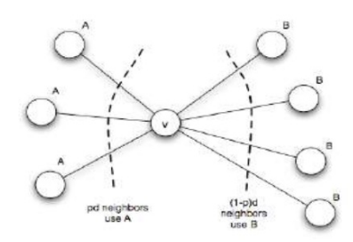
\includegraphics[width=0.6\textwidth]{netwroks.PNG}
    \caption{Graph of v's neighbours}
\end{figure}

\section{Literature Review}
\subsection{The wisdom, and madness, of crowds}
Let us first begin to under the idea behind Madness of the crowds by looking at some of the examples Mackay wrote about. In his article \cite{ref_lncs6}, Gregory A. Petsko talks about one of the widest known examples of herd mentality in history, Tulipomania. Mackay refers to this in the third chapter of his book. This example spoke about the time when around 1635, the popularity of possessing tulip bulbs reached nonsensical proportions and resulted in the price of a single bulb to be more expensive than gold \cite{ref_lncs7}. He then compares this senseless frenzy to modern day websites like Wikipedia that have rose to fame due to their ease in access and yet without any validation people seem to gobble up any information on these sites because of the fact that they’re popular and regardless of the fact that they can be edited by anyone, from anywhere. 

\subsection{Anxiety and Panic Buying Behaviour during COVID-19 Pandemic}
The COVID-19 pandemic has had a direct impact on buying patterns and has provoked the behavior of panic buying.
This also let to the sudden chase for a commodity that hardly got much attention, toilet paper. The paper by Leung, J. and authors on Anxiety and Panic Buying Behavior during COVID-19 Pandemic-A Qualitative Analysis of Toilet Paper Hoarding Contents on Twitter is about the Toilet paper shortage in a society which was affected by a global pandemic.
The bulk buying of toilet paper was observed in several countries such as the United States, Australia, Canada, United Kingdom, Singapore, Japan, Hong Kong and other cities \cite{ref_lncs2}.  
This paper talks about the influence of social media platforms such as twitter that creates havoc amongst people. It instills a constant fear by highlighting empty toilet paper shelves in the supermarkets. This results in out of stock situations when people buy large quantities. However there was no imminent shortage observed but empty shelves were a consequence of panic buying and hoarding. \\

Individuals resorted to panic buying because of the understanding of game theory since an individual’s pay-off in situations is impacted by the actions of others. This shortage can be explained using the concept of prisoner’s dilemma using game theory. There are two players, an individual A and the rest of the population.
They both have two choices, to panic buy all toilet paper or to act normally. If everyone acts normally, there will be toilet paper on the shop shelves, and people can relax and buy it as they need it. However, if person A buys more than normal and the rest do not then the chance that he would get the desired consumption of toilet paper. 
This would mean that A would get his stock piled up but it would lead to no toilet paper for the rest of the people to buy. The consequences would be the same if rest of the public panic buys and A does not.  When both players do not panic buy, they get the quantity that they require but the payoff is lower than when they would panic buy because there is a risk of shelves being empty in the future due to uncertain circumstances of the future. However, if both parties panic buy there is a chance that both will get more than enough storage for themselves but there is a greater chance of no toilet paper due to the sudden increased demand.
\\
\begin{center}
\begin{tabular}{ | c | c| c | } 
\hline
 & A panic buys &  A does not panic buy \\ 
\hline
Public panic buys  & (1, 1)  & (10, 0) \\ 
\hline
Public does not panic buy  & (0, 10)  & (5, 5) \\ 
\hline
\end{tabular}
\end{center}

According to the payoff matrix, if the public panic buys then for A to panic buy has a payoff of 1 rather than 0. Vice versa if public does not panic buy then a payoff of 10 is achieved if A panic buys. Thus, it will be more efficient and attractive for an individual to panic buy irrespective of what others do. It would be beneficial if both don’t do it but if one agent does it in fear of lack of stock then other individuals will also act in the same manner and run to stores. 

The paper helps demonstrate how an individual acts especially when they recognize that they have a better payoff. It highlights that madness of crowds exists in the market, even if it is a basic commodity such as toilet paper.   

\subsection{Pattern of panic-buying and its psycho-social correlates among Pakistani adults during COVID-19 pandemic}

On 30th October 2020, a case study was conducted to see patterns of panic-buying in Pakistani Adult because of the Covid 19 pandemic \cite{ref_lncs5}. We shall look at this study to understand the influence of Cascading Behavior displayed in a network and link it our study of the madness of crowds. In the study over 786 participants took part with over 59\% female population and a mean age of 26.6 years. The study took a a look at the hoarding tendencies and the act of panic buying that resulted in a shortage of stock across many stores. According to the paper, panic buying was defined as a crowd activity where people seek to buy the essential food and consumption supplies in bulk in the fear of not being left behind as others to the same. The study then correlated the Panic buying and Hoarding, to four psychological parameters, Severity of Covid (CA), Self Interest (SI), Social Responsibility (SR) and Social Trust (ST). Moreover, “It was hypothesized that more PBH will be associated with higher CA, greater SI, and reduced SR and ST.” The results of the study showed a significant positive correlation with Social Trust and Self Interest. 11.3\% if the survey population “feared supermarkets will run out of food”, while another 12.5\% believed that they stockpiled to prepare for a crisis in the fear than nothing will be available soon. It further states that “The element of SI was also positively correlated with PBH among the participants (p=0.02) \cite{ref_lncs5}”  


\begin{figure}[H]
    \centering
  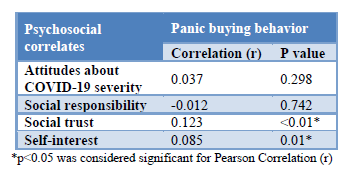
\includegraphics[width=0.8\textwidth]{Correlation.png}
    \caption{Frequency of bulk buying}
\end{figure}

\subsection{Introducing a Multi-Asset Stock Market to Test the Power of Investor Networks}
The behaviour of financial markets has frustrated, and continues to frustrate, investors and academics.
By utilizing a complex systems framework, researchers have discovered new fields of investigations that have provided a meaning insightful into the behavior of financial markets. Our case study \cite{ref_lncs3} discusses the use of agent-based models (ABMs) and network science to provide meaningful insights into the behaviour of financial markets.  This paper implemented artificial stock market using an Ising model-based agent-based model. The purpose of the model was to have the agents allocate their wealth between the risk-free and a risky asset. At each time step, the investors decided based on whether they wish to buy, hold, or sell more of the risky asset. Once investors made their investment decision, they transact via the artificial stock market, with a new price for the risky asset endogenously determined based on the relative demand and supply for the risky asset. Finally, investors reassess the level of trust they have in the information coming from the public source  and their network , dependent on whether it provided the correct advice. That is, if the information tells the agent to invest and the price subsequently increases, then the agent will increase the trust in that source. Alternatively, the trust will decline if the price falls following a buy signal from the information source. In this model, they used four different type of general network models, the Erdos-Renyi, Regular-ring lattice, Watts-Strogatz, and the Barabasi-Albert model. The values for the parameters used are mentioned in Table \ref{tab1} except the bias value of the bias towards network information,$c_1$ which was varied between $1$ and $4$ . 

    
\begin{table}[H]
\caption{Default settings used to test and verify the model}\label{tab1}
\begin{center}
    
\begin{tabular}{|l|l|}
\hline
\textbf{Variable}                            & \textbf{Setting} \\ \hline
Steps per run / Number of   runs per setting & $3000/50$         \\ \hline
Number of investors                          & 2500             \\ \hline
Conviction threshold                         & 2                \\ \hline
Market depth ($\lambda$)                             & 0.25             \\ \hline
Transaction ratio                            & 0.02             \\ \hline
Memory length ($\alpha$)                            & 0.95             \\ \hline
Initial bias to all   information            & 1                \\ \hline
\end{tabular}
\end{center}
\end{table}
The number of edges (5,000) and the average number of neighbours (4) were kept consistent across the different network structures. Therefore, any difference in the outcome was not influenced by the number of edges, but solely by the degree distribution of the networks. The default characteristics for each different network are summarised in Table 2. 
\begin{table}[H]
\caption{Default network characteristics}\label{tab2}
\begin{center}
\begin{tabular}{|c|c|}
\hline
\textbf{Network}             & \textbf{Key Characteristics}               \\ \hline
Lattice                      & Number of links per investor =  4          \\ \hline
\multirow{2}{*}{Small-world} & Number of   initial links per investor = 4 \\ \cline{2-2} 
                             & The probability of rewiring   = 0.10       \\ \hline
Erdos-Renyi                  & Probability of   connection = 0.0016       \\ \hline
\multirow{2}{*}{Scale-fee}   & Number of hubs = 10                        \\ \cline{2-2} 
                             & Probability of connection =   0.20         \\ \hline
\end{tabular}
\end{center}
\end{table}
\begin{figure}[H]
\centering
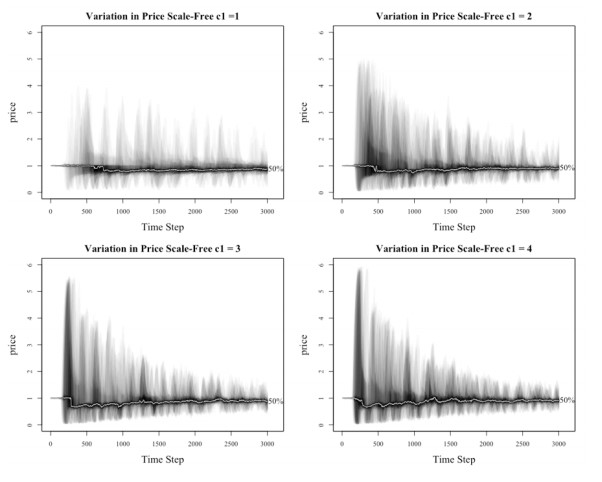
\includegraphics[width=\textwidth]{Fig5.jpg}
\caption{Lattice network with varying $c_1$ over time.} \label{fig1}
\end{figure}
The first key finding of this paper was that the network topology that investors form significantly affects the behavior of the market.The results from the lattice network starts to deviate in any meaningful manner from a price level of 1 when the level of c1 is greater than 2. The existence of bubbles and crashes, demonstrated by the price approaching 8 and 0, is seen when $c_1$ is equal to 4. The behavior of the scale-free network is materially different from the behavior of different network which as witnessed by the dramatic price movements regardless of the value of $c_1$.
\begin{figure}[H]
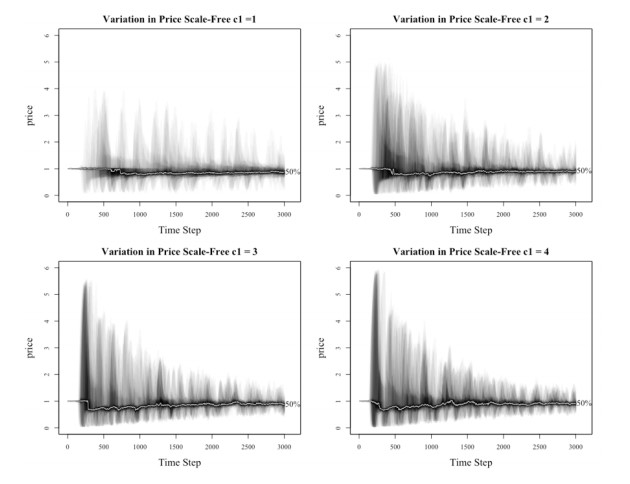
\includegraphics[width=\textwidth]{Fig6.jpg}
\caption{Scale free network with varying $c_1$ over time.} \label{fig2}
\end{figure}
\begin{figure}[H]
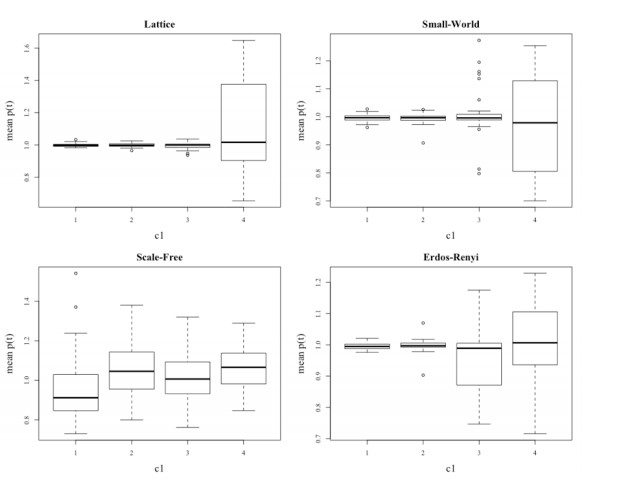
\includegraphics[width=\textwidth]{Fig7.jpg}
\caption{Box plots showing the mean prices with the various networks.} \label{fig3}
\end{figure}
Figure \ref{fig3} illustrates that as $c_1$ increases, the volatility in all the networks starts to increase. However, the level of volatility is not consistent across the networks, and this is the second finding of significance of this paper. The difference in the volatility of the networks is seen more clearly in Figure \ref{fig4}, which displays box plots of the standard deviation of the prices within the different scenarios.
\begin{figure}[H]
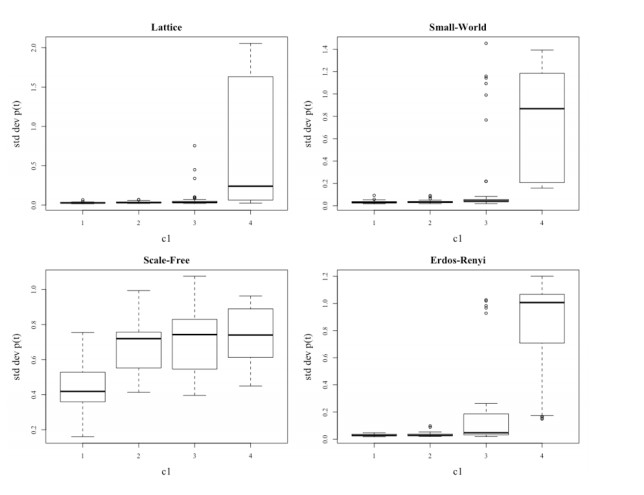
\includegraphics[width=\textwidth]{Fig8.jpg}
\caption{Box plots showing the standard deviation in prices with the various networks.} \label{fig4}
\end{figure}
This research paper gives us an insight about the role network dynamics play in the formation of the herds among investors in terms of their investment strategies. It is important to understand the reasons behind herd formation as it helps understand how and why bubbles form and collapse in financial markets.
\section{Applications in localised contexts}
\subsection{Panic buying groceries during the COVID-19 pandemic}
% Mentioning the survey results here. I guess
A cross-sectional survey-based study was carried out among the Pakistani adults during the 2ND wave of Covid-19 lockdown period in order to understand the groceries buying pattern during the pandemic. All participants self-selected themselves into an anonymous 5 minutes long online survey (via Google forms). At the beginning of the survey, participants were briefed about the purpose of the study and informed consent was taken. \\
The survey was taken in English and consisted of questions related to socio-demographic of the participants such as age, gender, marital status, profession, employment and number of family members. Panic buying was assessed by three items. Participants were required to indicate how they engaged in panic buying as the fear of scarcity grew high with a Yes/No/Maybe answer. And how frequently they bought groceries in bulk since the lockdown on a 5-point scale (1-5), where 1 indicated strongly disagreeing to bulk buying and 5 indicated strongly agreeing to bulk buying. While the third item was more of a descriptive question subjective to the participant that whether the mass hysteria forced people to change their buying and consumption patterns.\\
Out of 90 responses, there were more male(70.8\%) than female participants(29.2\%). About 78.7\% were adults aged between 18-30, 15.7\% aged between 31-50 and 5.6\% were 50+. As far as the employment and marital status is concerned, most of them were single(60.7\%) and employed(52.8\%).

\begin{center}
\begin{table} [H]
% \centering
\label{tab:my-table}
\begin{center}
\begin{tabular}{|c|l|l|}
\hline
\multicolumn{2}{|c|}{Socio-demographic variables} & Frequency ( N / \% ) \\ \hline
\multirow{3}{*}{Age}                & 18-30       & 70 / 78.7  \%        \\ \cline{2-3} 
                                    & 31-50       & 14 / 15.7\%          \\ \cline{2-3} 
                                    & 50+         & 5  / 5.6\%           \\ \hline
\multirow{2}{*}{Gender}             & Male        & 63 / 60.8\%          \\ \cline{2-3} 
                                    & Female      & 26 / 29.2\%          \\ \hline
\multirow{3}{*}{Marital Status}     & Single      & 54 / 60.7\%          \\ \cline{2-3} 
                                    & Married     & 33 / 37.1\%          \\ \cline{2-3} 
                                    & Other       & 2 / 2.2\%            \\ \hline
\multirow{2}{*}{Employment Status}  & Employed    & 47 / 52.8\%          \\ \cline{2-3} 
                                    & Unemployed  & 42 / 47.2\%          \\ \hline
\end{tabular}
\end{center}

\caption{Socio-demographic variables of the study participants (n=89)}
\end{table}
\end{center}
The participants also had a variety of professional backgrounds dominated mainly by students(40\%) as shown below: 
\begin{figure}[H]
    \centering
  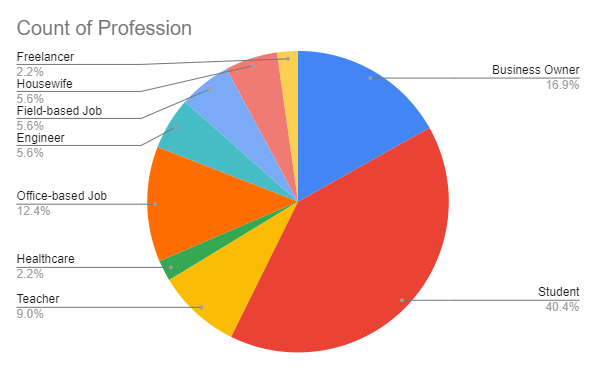
\includegraphics[width=0.7\textwidth]{graphs/profession2.PNG}
    \caption{Pie chart of Professions}
\end{figure}

There was another comparison drawn based on the number of family members each participant had. Of our study sample, 25.8\%(23) have five family members, while around 1\% participants had 1 and 2.2\%(2) had maximum of 11 family members. 
\begin{figure}[H]
    \centering
  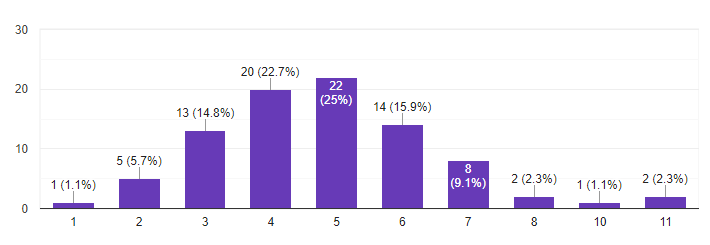
\includegraphics[width=0.8\textwidth]{graphs/family_members.PNG}
    \caption{Bar chart of Family members}
\end{figure}
In particular, 59.1\%(52) of the participants did not engaged in panic buying at all, while 22.7\%(21) hoarded supplies a few times or more than that. Of all the participants, only 58.4\%(52) strongly disagreed that they bought supplies in bulk than usual while only 31.5\%(28) partially agreed to have bought more food and supplies due to the pandemic.
\begin{figure}[H]
    \centering
  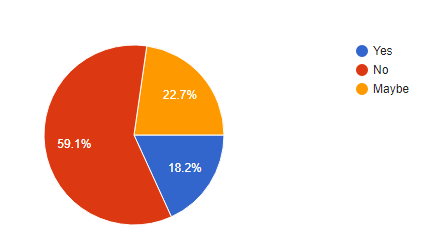
\includegraphics[width=0.8\textwidth]{graphs/grocery.PNG}
    \caption{Engagement in panic as a fear of scarcity}
\end{figure}
\begin{figure}[H]
    \centering
  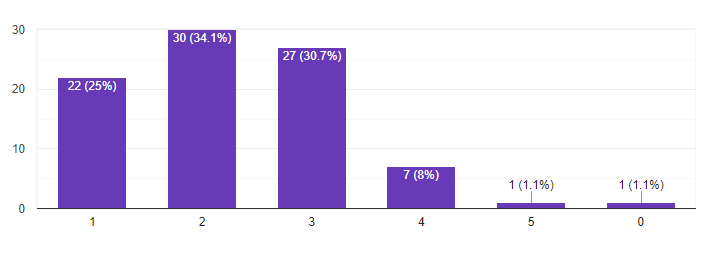
\includegraphics[width=0.8\textwidth]{graphs/bulk.PNG}
    \caption{Bar chart of bulk buying}
\end{figure}



\subsection{What Causes Stock Market Volatility in Pakistan? Evidence from the Field}
Our case study \cite{ref_lncs4} examined the presence of volatility at the Karachi Stock Exchange (KSE) by fitting Exponential Generalized Autoregressive Conditional Heteroskedasticity (EGARCH) model to 25 years’ index data. In this study they  found that the ARCH effects are present in the data indicating the stock market cluster volatility during the period under study. In addition to, they also found persistent high volatility in the stock market and presence of negative leverage effect. After confirming the presence of volatility in the stock market, using literature reviews and preliminary interviews. They collected and analyzed the primary data from 246 individual investors of stock market and 28 brokers listed with KSE. The following factors were identified for the causes of volatility in the stock market. 
\begin{itemize}
    \item[1.] News stories in the media
    \item[2.] Forecasts of the analysts
    \item[3.] Change in earnings of listed companies
    \item[4.] Herd Behaviour
    \item[5.] Government policies
    \item[6.] Political situation
    \item[7.] Manipulation by big investors
\end{itemize}
Afterwards,investors were asked to the above seven factors in on a scale from 1 (least important) to 7 (most important). Analytic Hierarchy Process (AHP) was then used to find the relative weights and ranking of these seven factors by adopting the following procedure. The results that were obtained can be seen in Figure \ref{fig8}
\begin{figure}[H]
    \centering
  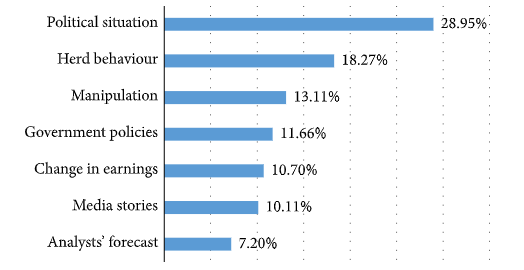
\includegraphics[width=0.8\textwidth]{AHP.png}
    \caption{AHP results for the factors causing market volatility}
    \label{fig8}
\end{figure}
The results suggest that political situation and herd behavior are the most important factors to have major impact on the stock market in terms of volatility. This is an important case study for our paper confirms the presence of clustered volatility in the market which is an indicator of asset bubbles. Another important finding of this case study was that market volatility cannot be solely attributed toward political instability. We will use the findings in this study and insights gained by the ABM model of the Artificial Stock Market to determine the underlying network structure which is the driving force for this herding behavior.
% Talk about the existing studies and there methodology//
\section{Discussion and Conclusion}
% Discuss the survey results and findings regarding Panic Buying

When looked at a perspective of the madness of crowds, it is not too difficult to understand that while there were no hypothesized threats of supermarkets running out of stocks or a shortage in food supplies, the fear of being left behind and the motivation of self interest had driven some people to panic buy. This then resulted in a cascade where people who saw others hoard supplies were inclined to act in self interest and exhibit the same behavior.

For our report we conducted a similar survey to gauge the trends of panic buying and we received a similar outcome where 31.5\% of the population partially agreed to have bought more supplies than usual due to the pandemic. According to the survey, more than half of the participants agreed in their detailed answers to the statement that mass hysteria forced people to change their buying and consumption patterns. Almost all of them had similar reasoning that the general public were under the impression that the stores might run out of stocks and supplies in case of times of uncertainty and prolonged lockdown. People also bought more than they needed because they were afraid of going out again and again so better be safe than sorry. While a few people disagreed with the notion and believed that buying is more impacted by income constraints and that lockdown caused more damage economically that the people buying patterns were restricted to essentials only.

The survey outlined a relationship between panic buying,  self-interest and social trust. An irrational behaviour is demonstrated where individuals act out of fear. The same pattern can be observed in the case study which talks about hoarding of toilet paper. Individuals resorted to panic buying, according to the prisoners dilemma, where they had a higher payoff regardless of what others did because of their self-interest that was ignited due to fear. In essence, this goes to testify that how an irrational collective behaviour such as panic buying can occur as a result of the interaction among rational agents. 

Now we will focus on our second local case study, the Karachi Stock Exchange. In the case study on the Karachi Stock Exchange , index data of over a period of 25 years was analysed which confirmed the presence of clustered volatility \cite{ref_lncs4}. In addition, they conducted surveys and literature reviews and then identified the political instability and herding behavior as the two main possible factors that were causing the clustered volatility. In \cite{ref_lncs3}, the results obtained also clustered volatility. However, there is one caveat. The EGARCH model assumes that the relative differences are Gaussian distribution \cite{ref_lncs3} clustered volatility indicated a leptokurtic distribution. Consequently, the insights that we were able to obtain from the agent-based model of the Artificial stock market cannot be directly applied in the context of the Karachi Stock Exchange. 

Although, based on these ideas we can speculate that the degree distribution of the KSE investor network can be approximated by a power law. If the network indeed follows a power-law distribution, then we know that there are hubs in the networks. Examples of hubs could include rating agencies, brokers, large pension funds, and renowned stock pickers. If these hubs became correlated then the rest of the investing universe would have little choice but to follow. This means that the hubs can modify the trends in the market such that it suits their interests. If a major investor buys the stocks of a particular company, the other investors will follow soon start buying that stock as well causing its price to rise. The major investors can then sell these stocks before their price and therefore maximize their profit. This shows that if rational agents have a bias towards the network information, and they modify their actions based on their neighbor's actions, irrational collective behavior such as asset bubbles can occur.

There are multiple takeaways in this report. The first takeaway is that the major investors have a significant impact on the output from the financial markets so their behavior can give an insight how the market will perform. The second takeaway is that since information plays a significant role in how investors decide their investment strategy, the source of the information should be given due consideration. Information asymmetry in the markets means that the losses can be quite more than one's expectation. The final and the most important takeaway is that although the bubbles are not something that happens on the regular basis we are incapable of predicting when the next bubble will occur or identifying a bubble until it actually happens. Bubbles only form when the bias investor bias towards network information was increased beyond a critical threshold. 

The results achieved in this report are in agreement with our hypothesis that information cascade leads to herding behaviour which then results in the manifestation of the phenomena, Madness of the Crowds






\newpage


\begin{thebibliography}{8}


\bibitem{ref_lncs1}
N. E. Glynatsi and V. A. Knight, A bibliometric study of research topics, collaboration and centrality in the Iterated Prisoner’s Dilemma. \url{http://export.arxiv.org/}.

\bibitem{ref_lncs2}
 Leung, J. , Chung, J.Y.C. , Tisdale, C. , Chiu, V. , Lim, C.C.W. , Chan, G Anxiety and Panic Buying Behaviour during COVID-19 Pandemic-A Qualitative Analysis of Toilet Paper Hoarding Contents on Twitter. Int. J. Environ. Res. Public Health 2021, 18, 1127. \doi{10.3390/ijerph18031127}
 
\bibitem{ref_lncs3}

Oldham, M.: Introducing a Multi-Asset Stock Market to Test the Power of Investor Networks , Journal of Artificial Societies and Social Simulation \textbf{20}(4), 13(2017) \url{http://jasss.soc.surrey.ac.uk/20/4/13.html} \doi{10.18564/jasss.3497}
		
\bibitem{ref_lncs4}
Ghufran, Bushra et al. What Causes Stock Market Volatility in Pakistan? Evidence from the Field.Economics Research International 2016 (2016): 1-9.
% Author, F.: Article title. Journal \textbf{2}(5), 99--110 (2016)

\bibitem{ref_lncs5}
Abbas, Kiran et al. Pattern of panic-buying and its psychosocial correlates among Pakistani adults during COVID-19 pandemic. International Journal of Research in Medical Sciences \textbf{8}12,4206-4211,2020. \url{https://www.msjonline.org/index.php/ijrms/article/view/8906} \doi{10.18203/2320-6012.ijrms20205290}

\bibitem{ref_lncs6}
Petsko, G.A. The wisdom, and madness, of crowds. Genome Biology  \textbf{9}(112),2008. \doi{10.1186/gb-2008-9-11-112}

\bibitem{ref_lncs7}
Mackay, Charles. Extraordinary Popular Delusions and the Madness of Crowds. New York: L.C. Page, 1932. Print.



\end{thebibliography}
\newpage
\appendix
\section{Survey questions}
\begin{figure}[H]
    % \centering
  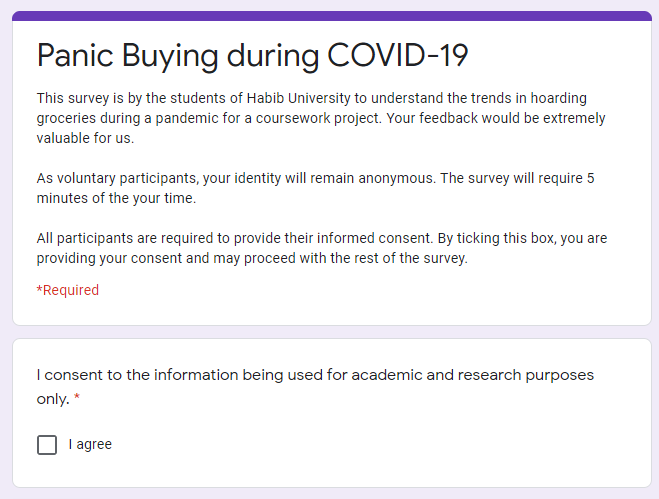
\includegraphics[width=0.8\textwidth]{survey-pg1.PNG}
\end{figure}
\begin{figure}
  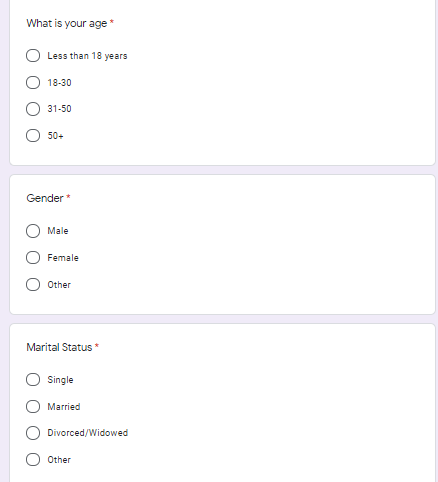
\includegraphics[width=0.8\textwidth]{survey-pg2.PNG}
  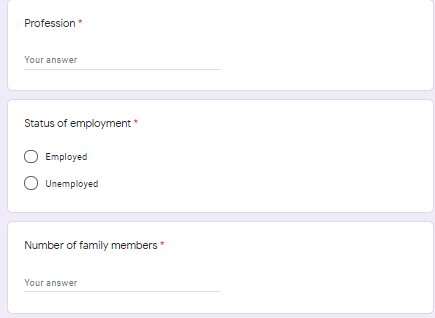
\includegraphics[width=0.8\textwidth]{survey-pg3.PNG}
\end{figure}
\newpage
\begin{figure}
  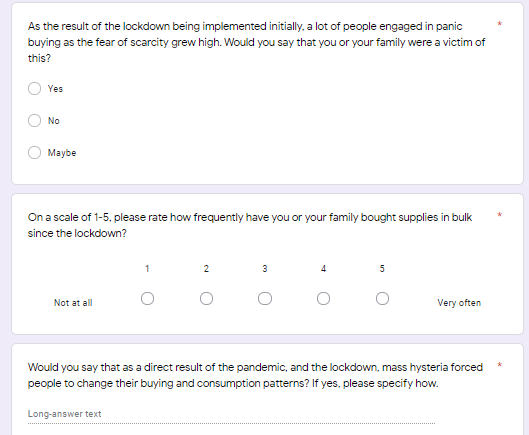
\includegraphics[width=0.8\textwidth]{survey-pg4.PNG}
    % \caption{AHP results for the factors causing market volatility}
    % \label{fig8}
\end{figure}

\end{document}
